\documentclass[12pt,a4paper]{report}

% Packages for formatting, images, and math
\usepackage[utf8]{inputenc}
\usepackage[T1]{fontenc}
\usepackage{geometry}
\geometry{a4paper, margin=1in}
\usepackage{graphicx}
\usepackage{float}
\usepackage{amsmath}
\usepackage{booktabs}
\usepackage{titlesec}
\usepackage{setspace}

% Set font to Times New Roman
\usepackage{mathptmx}

% Format chapter headings
\titleformat{\chapter}[display]
  {\normalfont\huge\bfseries}{\chaptertitlename\ \thechapter}{20pt}{\Huge}
\titlespacing*{\chapter}{0pt}{-20pt}{20pt}

\begin{document}

% ---------------- TITLE PAGE ----------------
\begin{titlepage}
    \begin{center}
        \vspace*{1cm}
        
        \Huge
        \textbf{Field Oriented Control (FOC) for a 3-Phase Induction Motor}
        
        \vspace{1.5cm}
        
        \Large
        \textit{Project Report Submitted in partial fulfilment of the requirements for the degree of\\
        Bachelor of Technology from Maulana Abul Kalam Azad University of Technology, West Bengal\\
        (formerly known as West Bengal University of Technology)}
        
        \vspace{1.5cm}
        
        \textbf{By}\\
        \vspace{0.5cm}
        \textbf{Surja Mondal (Roll No. 34901622011)}\\
        \textbf{Joydip Karmakar (Roll No. 34901622014)}\\
        \textbf{Angsu Priya Roy (Roll No. 34901622020)}\\
        \textbf{Hirak Sinha (Roll No. 34901622042)}\\
        \textbf{Keshab Sarkar (Roll No. 34901622044)}\\
        \textbf{Jibitesh Basunia (Roll No. 34901622045)}
        
        \vspace{1.5cm}
        
        \textit{Under the Guidance of}\\
        \vspace{0.5cm}
        Prof. Deepjyoti Santra
        
        \vfill
        
        \Large
        \textbf{Department of Electrical Engineering}\\
        \textbf{Cooch Behar Government Engineering College}\\
        \textbf{Cooch Behar, West Bengal}\\
        \vspace{0.5cm}
        \textbf{2026}
        
    \end{center}
\end{titlepage}

% ---------------- CERTIFICATES ----------------
\chapter*{Certificate of Recommendation}
\addcontentsline{toc}{chapter}{Certificate of Recommendation}
It is hereby recommended to consider the project report entitled "Comprehensive Analysis of Field Oriented Control (FOC) for a 3-Phase Induction Motor" submitted by Surja Mondal, Joydip Karmakar, Angsu Priya Roy, Hirak Sinha, Keshab Sarkar, and Jibitesh Basunia for partial fulfillment of the requirements for the award of the degree of Bachelor of Technology in Electrical Engineering from Maulana Abul Kalam Azad University of Technology (formerly known as West Bengal University of Technology).

\vspace{3cm}
\noindent
\begin{tabular}{@{}p{0.5\linewidth}p{0.5\linewidth}@{}}
------------------------------ & ------------------------------- \\
Prof. Deepjyoti Santra & Prof. Atanu Maji  \\
Project Guide & (Head of Electrical Engg. Department)
\end{tabular}

\chapter*{Certificate of Approval}
\addcontentsline{toc}{chapter}{Certificate of Approval}
It is hereby approved that the project report entitled \textbf{"Comprehensive Analysis of Field Oriented Control (FOC) for a 3-Phase Induction Motor"} submitted by Surja Mondal, Joydip Karmakar, Angsu Priya Roy, Hirak Sinha, Keshab Sarkar, and Jibitesh Basunia for partial fulfilment of the requirements for the award of the degree of Bachelor of Technology in Electrical Engineering from Maulana Abul Kalam Azad University of Technology (formerly known as West Bengal University of Technology).

\vspace{1.5cm}
\noindent\textbf{Board of Examiners}

\vspace{1.5cm}
\noindent 1. ------------------------------------

\vspace{1cm}
\noindent 2. ------------------------------------

% ---------------- ACKNOWLEDGEMENT ----------------
\chapter*{Acknowledgement}
\addcontentsline{toc}{chapter}{Acknowledgement}
We would like to express our gratitude to Prof. Deepjyoti Santra for their guidance, support, and knowledge throughout this project.

We are also thankful to the Head of the Electrical Engineering Department, Prof. Atanu Maji , for providing the necessary facilities to complete this work.

Furthermore, we extend our thanks to our colleagues and the laboratory staff of Cooch Behar Government Engineering College for their cooperation.

Finally, we would like to thank our families for their encouragement.

\vspace{2cm}
\noindent
\begin{tabular}{@{}p{0.5\linewidth}p{0.5\linewidth}@{}}
\rule{6cm}{0.5pt} & \rule{6cm}{0.5pt} \\
\textbf{Surja Mondal} & \textbf{Joydip Karmakar} \\
(Roll No. 34901622011) & (Roll No. 34901622014) \\[2cm]

\rule{6cm}{0.5pt} & \rule{6cm}{0.5pt} \\
\textbf{Angsu Priya Roy} & \textbf{Hirak Sinha} \\
(Roll No. 34901622020) & (Roll No. 34901622042) \\[2cm]

\rule{6cm}{0.5pt} & \rule{6cm}{0.5pt} \\
\textbf{Keshab Sarkar} & \textbf{Jibitesh Basunia} \\
(Roll No. 34901622044) & (Roll No. 34901622045) \\
\end{tabular}

% ---------------- FRONT MATTER ----------------
\renewcommand{\contentsname}{\textit{Contents}}
\tableofcontents
\listoffigures
\listoftables

\chapter*{List of Principal Symbols and Acronyms}
\addcontentsline{toc}{chapter}{List of Principal Symbols and Acronyms}
\begin{itemize}
    \item \textbf{FOC:} Field Oriented Control
    \item \textbf{IFOC:} Indirect Field Oriented Control
    \item \textbf{SVPWM:} Space Vector Pulse Width Modulation
    \item \textbf{PI:} Proportional-Integral
    \item \textbf{$V_s$:} Stator Voltage
    \item \textbf{$i_{ds}$:} Direct-axis stator current (Flux-producing)
    \item \textbf{$i_{qs}$:} Quadrature-axis stator current (Torque-producing)
    \item \textbf{$\psi_r$:} Rotor flux linkage
    \item \textbf{$T_e$:} Electromagnetic Torque
    \item \textbf{$\theta_e$:} Electrical rotor flux angle
    \item \textbf{$\omega_m$:} Mechanical rotor speed
    \item \textbf{$\omega_{sl}$:} Slip frequency
\end{itemize}

\chapter*{Abstract}
\addcontentsline{toc}{chapter}{Abstract}
This report provides a component-level technical analysis of the Simulink model \\ VECTOR\_CONTROL\_FOC\_OF\_IM.slx, which implements an Indirect Field Oriented Control (IFOC) architecture for a 50 HP Squirrel-Cage Induction Motor.

Intended as an instructional document for electrical machines and drives coursework, this report deconstructs the theoretical and practical frameworks within the simulation. It establishes the plant's equivalent circuit parameters and dynamic modelling. The analysis explores the coordinate transformations (Forward and Reverse Clarke and Park) required to map stationary three-phase variables into a synchronously rotating $d-q$ reference frame.

By examining the decoupling equations, the report demonstrates how IFOC achieves independent regulation of rotor flux and electromagnetic torque, mirroring the dynamics of a separately excited DC machine. Furthermore, the document evaluates the discrete-time closed-loop control strategy, detailing the tuning parameters and anti-windup mechanisms of the cascaded Proportional-Integral (PI) controllers used in the outer speed and inner current loops. Finally, the report analyses the Space Vector Pulse Width Modulation (SVPWM) synthesis used to drive the three-phase inverter, noting its effect on DC bus utilisation and total harmonic distortion (THD).

This analysis connects electromechanical theory with digital control implementation.

% ---------------- CHAPTER 1 ----------------
\chapter{INTRODUCTION}

\begin{figure}[H]
\centering
\includegraphics[width=0.9\textwidth]{0.png}
\caption{Overall Simulink Architecture of Field Oriented Control of IM}
\end{figure}

\section{Introduction}
Traditionally, the control of induction machines was dominated by scalar methods, such as constant Volts-per-Hertz (V/f) control. Scalar control governs the magnitude and frequency of the applied voltage and currents, independent of the spatial orientation of the electromagnetic fields. Consequently, scalar methods exhibit delayed transient responses, cross-coupling effects, and an inability to independently regulate torque and flux during dynamic state changes.

Field Oriented Control (FOC), also known as Vector Control, is an AC machine drive control method that addresses the limitations of scalar control. The objective of FOC is to emulate the decoupled control dynamics of a separately excited DC motor. In a traditional DC machine, the field flux and the armature flux are maintained in a state of spatial orthogonality (perpendicularity) by the mechanical commutator. This decoupling allows the field current and armature current to be manipulated independently to control magnetic flux and electromagnetic torque, respectively.

\section{Review of Previous Works (Literature Review)}
The evolution of AC motor control has progressed significantly. Early literature focused on addressing the coupled, non-linear multivariable nature of induction motors. Vector Control methodology introduced coordinate transformations (Clarke and Park) to project time-varying AC parameters into a synchronous, DC-like reference frame.

While Direct FOC techniques emerged first, relying on physical air-gap sensors for flux measurement, the industry moved toward Indirect Field Oriented Control (IFOC). IFOC mathematically estimates the rotor flux angle by compounding the measured rotor speed with a calculated slip frequency, providing a method used in industrial drives.

To replicate orthogonal decoupling in a three-phase AC induction machine, FOC treats the multi-phase stator currents as spatial vectors. Through mathematical coordinate transformations—namely the Clarke and Park transforms—the time-varying, three-phase AC variables ($i_a, i_b, i_c$) are projected onto a two-dimensional, synchronously rotating reference frame ($d-q$ axes). Because this reference frame rotates at the same synchronous speed as the machine's magnetic field, the sinusoidal AC quantities are transformed into DC steady-state values, allowing for the implementation of standard Proportional-Integral (PI) control loops.

By aligning the direct-axis ($d$-axis) of this rotating frame with the rotor flux linkage vector, the overall stator current is mathematically decomposed into two independent, orthogonal components:

\textbf{Flux-Producing Component ($i_{ds}$):} The direct-axis stator current is constrained by the control algorithm to align with the rotor flux linkage vector ($\psi_r$). In this oriented reference frame, $i_{ds}$ acts analogously to the field excitation current ($I_f$) in a separately excited DC motor; it is responsible for establishing and maintaining the internal magnetisation of the induction machine.

Under steady-state conditions, the relationship is linear: the rotor flux magnitude is governed by $\psi_r = L_m i_{ds}$. In the constant-torque region of operation (below base speed), $i_{ds}$ is maintained at a constant nominal value. Conversely, in the constant-power region (above base speed), $i_{ds}$ is attenuated to facilitate ``field weakening,'' reducing the back-EMF to allow further speed increases within the inverter's voltage limit.

\textbf{Torque-Producing Component ($i_{qs}$):} The quadrature-axis stator current is maintained at a $90^\circ$ electrical angle relative to the rotor flux axis. Because the machine's flux is isolated onto the $d$-axis ($\psi_{qr} = 0$), the cross-product interaction that generates mechanical force relies on this orthogonal $q$-axis current. It operates analogously to the armature current ($I_a$) in a DC motor.

The developed electromagnetic torque can be expressed via the decoupled equation:
\begin{equation}
T_e = \frac{3}{2} \left(\frac{P}{2}\right) \frac{L_m}{L_r} \psi_r i_{qs}
\end{equation}

[Calculation Execution] Substituting the motor parameters: $P = 4$, $L_m = 34.7 \text{ mH} = 0.0347 \text{ H}$, $L_r = L_{lr} + L_m = 0.8 \text{ mH} + 34.7 \text{ mH} = 35.5 \text{ mH} = 0.0355 \text{ H}$, and assuming nominal flux $\psi_r = 0.96 \text{ Wb}$:
\begin{equation}
T_e = \frac{3}{2} \left(\frac{4}{2}\right) \left(\frac{0.0347}{0.0355}\right) (0.96) \cdot i_{qs}
\end{equation}
\begin{equation}
T_e = 3 \times (0.9775) \times (0.96) \cdot i_{qs}
\end{equation}
\begin{equation}
T_e \approx 2.8152 \cdot i_{qs} \text{ N}\cdot\text{m}
\end{equation}
This establishes a linear torque constant of $2.8152 \text{ N}\cdot\text{m/A}$ for the $q$-axis current. Because the rotor flux $\psi_r$ is held constant by the independent $d$-axis control loop, the electromagnetic torque $T_e$ is directly and linearly proportional to $i_{qs}$.

This spatial decoupling allows the induction motor to respond to step changes in torque demand, reducing the transient delay and cross-coupling dynamics of scalar (V/f) control methods.

A requirement for FOC is the real-time determination of the rotor flux angle ($\theta_e$) to execute the Park and Inverse-Park transformations. The Simulink architecture analysed in this report utilises \textbf{Indirect Field Oriented Control (IFOC)}. Rather than relying on physical Hall-effect sensors embedded in the air gap or state observers to directly measure the flux (Direct FOC), the IFOC scheme calculates the required flux angle. It achieves this by taking the measured mechanical rotor speed and adding it to a calculated, feedforward slip frequency.

\section{Objective and Motivation}
The primary objective of this project is to analyse and document a functional Simulink model of an IFOC system for a 3-phase induction motor. The motivation is to bridge theoretical electromechanical equations with discrete-time digital control logic. By deconstructing the model, the project demonstrates how continuous-time theory is translated into a simulated DSP environment for the regulation of torque and flux.

\section{Scope of Present Work}
The scope of this report covers the mathematical and functional breakdown of the \\VECTOR\_CONTROL\_FOC\_OF\_IM.slx Simulink model. This includes the identification of the 50 HP Squirrel-Cage Induction Motor plant parameters, the derivation of the $d-q$ decoupling equations, the tuning of the discrete PI control loops, and the execution logic of the Space Vector Pulse Width Modulation (SVPWM) algorithm. Hardware implementation is considered future scope and is beyond the bounds of this simulation-based analysis.

% ---------------- CHAPTER 2 ----------------
\chapter{INDUCTION MOTOR PLANT PARAMETERS AND DYNAMIC MODELLING}

The electromechanical plant governed by this control architecture is a three-phase Squirrel-Cage Induction Motor (SCIM). 

From a control perspective, the squirrel-cage design means the rotor currents and rotor flux linkages are physically inaccessible and cannot be directly measured. Consequently, the control strategy relies on a mathematical model of the machine, dictated by its equivalent circuit parameters.

Based on the model's initialisation routines and the machine block mask configurations, the motor is defined by the ratings and parameters summarised in Table 2.1.

\begin{figure}[H]
\centering
\includegraphics[width=0.6\textwidth]{2.jpg}
\caption{Model Initialization Function (InitFcn) showing Plant Parameters}
\end{figure}

\begin{table}[H]
\centering
\caption{Squirrel-Cage Induction Motor Nominal Ratings and Equivalent Circuit Parameters}
\begin{tabular}{@{}llc@{}}
\toprule
\textbf{Parameter Description} & \textbf{Symbol} & \textbf{Value} \\ \midrule
\textbf{Nominal Ratings} & & \\
Nominal Power & $S$ & 50 HP (37.3 kW) \\
Stator Line-to-Line Voltage & $V_s$ & 460 V \\
Nominal Frequency & $f$ & 50 Hz \\
Number of Poles & $P$ & 4 (2 Pole Pairs) \\
Synchronous Speed & $N_s$ & 1500 RPM \\ \midrule
\textbf{Electrical Parameters (Per Phase)} & & \\
Stator Resistance & $R_s$ & 0.087 $\Omega$ \\
Rotor Resistance (Referred to Stator) & $R_r$ & 0.228 $\Omega$ \\
Stator Leakage Inductance & $L_{ls}$ & 0.1 mH \\
Rotor Leakage Inductance (Referred) & $L_{lr}$ & 0.8 mH \\
Magnetizing Inductance & $L_m$ & 34.7 mH \\ \midrule
\textbf{Mechanical Parameters} & & \\
Moment of Inertia & $J$ & 0.662 kg·m² \\
Viscous Friction Coefficient & $F$ & 0.1 N·m·s/rad \\ \bottomrule
\end{tabular}
\end{table}

\begin{figure}[H]
\centering
\includegraphics[width=0.8\textwidth]{3.jpg}
\caption{ABC to DQ Transformation and IM Mathematical Model Subsystem}
\end{figure}

\begin{figure}[H]
\centering
\includegraphics[width=0.9\textwidth]{4.jpg}
\caption{Internal Structure of the IM Mathematical Model}
\end{figure}

\section{Significance of Electrical Parameters in FOC}
In Vector Control, these parameters shape the dynamic transient response of the decoupling matrices. From the values provided, the lumped self-inductances of the stator ($L_s$) and rotor ($L_r$) are derived:
\begin{equation}
L_s = L_{ls} + L_m = 0.1 \text{ mH} + 34.7 \text{ mH} = 34.8 \text{ mH}
\end{equation}
\begin{equation}
L_r = L_{lr} + L_m = 0.8 \text{ mH} + 34.7 \text{ mH} = 35.5 \text{ mH}
\end{equation}

Converting the inductances to Henrys for base SI unit compatibility:
\begin{equation}
L_s = 34.8 \times 10^{-3} \text{ H} = 0.0348 \text{ H}
\end{equation}
\begin{equation}
L_r = 35.5 \times 10^{-3} \text{ H} = 0.0355 \text{ H}
\end{equation}

A required parameter in Indirect Field Oriented Control (IFOC) is the \textbf{rotor time constant ($\tau_r$)}, defined as:
\begin{equation}
\tau_r = \frac{L_r}{R_r} = \frac{35.5 \times 10^{-3}}{0.228} \approx 0.1557 \text{ seconds}
\end{equation}

In the IFOC feedforward slip-calculation pathway, the slip frequency ($\omega_{sl}$) is computed continuously as a function of the torque-producing current reference ($i_{qs}^*$) and this time constant. If the value of $R_r$ deviates during operation (e.g., due to thermal heating of the rotor bars), $\tau_r$ will change, leading to \textbf{detuning}. Detuning causes spatial misalignment between the expected and actual $d-q$ axes, resulting in cross-coupling where torque commands perturb the machine flux.

The machine's \textbf{total leakage factor ($\sigma$)}, which dictates the maximum rate of change of stator currents, is calculated as:
\begin{equation}
\sigma = 1 - \frac{L_m^2}{L_s L_r} \approx 1 - \frac{(34.7)^2}{(34.8)(35.5)} \approx 0.025
\end{equation}
This magnetic relationship ($\sigma \ll 1$) requires high-gain current loops to force the stator currents to track the FOC references.

\begin{figure}[H]
\centering
\includegraphics[width=0.8\textwidth]{5.jpg}
\caption{Dynamic State-Space Modeling of the $d$-axis Stator Current ($I_{ds}$)}
\end{figure}

\section{Mechanical Dynamics and Speed Loop Tuning}
The mechanical parameters—the moment of inertia ($J = 0.662 \text{ kg}\cdot\text{m}^2$) and the viscous friction coefficient ($F = 0.1 \text{ N}\cdot\text{m}\cdot\text{s/rad}$)—govern the low-frequency dynamics of the plant. While the electrical dynamics operate on the order of milliseconds, the mechanical dynamics operate on the order of tenths of seconds or slower. This temporal separation is the justification for the cascaded control architecture in this model, where an outer speed loop provides the torque command ($T_e^*$) to the inner current loops.

The mechanical equation of motion that dictates the rotor's dynamic trajectory is governed by:
\begin{equation}
T_e - T_L = J \frac{d\omega_m}{dt} + F\omega_m
\end{equation}
Substituting the mechanical parameters of the 50 HP motor:
\begin{equation}
T_e - T_L = 0.662 \frac{d\omega_m}{dt} + 0.1 \cdot \omega_m
\end{equation}
where $T_e$ is the developed electromagnetic torque, $T_L$ is the applied load torque, and $\omega_m$ is the mechanical rotor speed in rad/s.

To tune the outer Proportional-Integral (PI) speed controller, the plant is analysed in the complex frequency domain. Assuming the load torque $T_L$ acts as an independent disturbance ($T_L = 0$ for the primary plant transfer function), taking the Laplace transform of the mechanical equation yields:
\begin{equation}
\frac{\omega_m(s)}{T_e(s)} = \frac{1}{Js + F} = \frac{1}{0.662s + 0.1}
\end{equation}

This first-order transfer function indicates the mechanical plant acts as a low-pass filter. The inertia of the 50 HP motor provides kinetic energy storage that attenuates high-frequency torque ripples generated by the discrete switching of the SVPWM inverter. However, this inertia imposes an upper limit on the achievable bandwidth of the speed control loop.

The outer speed PI controller must be tuned to address this pole:
\begin{itemize}
    \item \textbf{Proportional Gain ($K_p$):} Provides the control effort to overcome the inertial mass ($J$) during transient speed changes.
    \item \textbf{Integral Gain ($K_i$):} Addresses steady-state tracking error and rejects steady-state load torque disturbances ($T_L$) applied to the shaft.
\end{itemize}

In practice, the speed loop bandwidth is constrained to be at least one decade slower than the inner $q$-axis current loop bandwidth. This frequency separation ensures that the inner loop appears as a gain of $1$ from the perspective of the outer loop.

% ---------------- CHAPTER 3 ----------------
\chapter{CONTROL SYSTEM ARCHITECTURE AND DISCRETE-TIME EXECUTION}

The Simulink model is architected around cascading subsystems that execute the Indirect Field Oriented Control (IFOC) algorithm. A parameter governing this digital control system is the fundamental sample time, set to $T_s = 2 \, \mu s$. This execution rate (equivalent to a 500 kHz update frequency) ensures that the discrete-time z-domain implementation introduces minimal phase delay. This temporal granularity is required for the synthesis of the Space Vector PWM signals and stability in the inner current regulation loops.

\begin{figure}[H]
\centering
\includegraphics[width=0.9\textwidth]{8.jpg}
\caption{FOC Control Architecture Schematic}
\end{figure}

\section{Coordinate Transformations: The Mathematical Foundation of FOC}
FOC resolves the limitation of standard AC linear controllers: the inability of a standard Proportional-Integral (PI) controller to track a time-varying sinusoidal reference without a steady-state magnitude and phase error. By transforming the time-varying, three-phase AC stator variables into a synchronously rotating $d-q$ reference frame, FOC mathematically forces these alternating signals to appear as DC quantities. This allows PI controllers to achieve zero steady-state error.

\begin{figure}[H]
\centering
\includegraphics[width=0.9\textwidth]{10.jpg}
\caption{Overall Reference Frame Transformation Process}
\end{figure}

\textbf{Forward Clarke Transform (Stationary $3 \to 2$ Projection):} The initial stage of the vector control algorithm simplifies the three-phase AC system by projecting the measured stator phase currents ($i_a, i_b, i_c$) onto an equivalent two-dimensional orthogonal reference frame ($\alpha-\beta$ axes). In a star-connected induction motor without a neutral return path, Kirchhoff's current law dictates that the sum of the phase currents is zero ($i_a + i_b + i_c = 0$). Consequently, the zero-sequence homopolar component ($i_0$) is zero and discarded.

To ensure that the peak amplitude of the phase currents is preserved in the two-phase system, the model utilises the amplitude-invariant Clarke transformation matrix:
\begin{equation}
\begin{bmatrix} i_\alpha \\ i_\beta \end{bmatrix} = \frac{2}{3} \begin{bmatrix} 1 & -\frac{1}{2} & -\frac{1}{2} \\ 0 & \frac{\sqrt{3}}{2} & -\frac{\sqrt{3}}{2} \end{bmatrix} \begin{bmatrix} i_a \\ i_b \\ i_c \end{bmatrix}
\end{equation}

\begin{figure}[H]
\centering
\includegraphics[width=0.7\textwidth]{11.png}
\caption{Forward Clarke Transformation Simulink Block}
\end{figure}
\begin{figure}[H]
\centering
\includegraphics[width=0.7\textwidth]{12.jpg}
\caption{Vector Representation of the Clarke Transform}
\end{figure}

Assuming instantaneous balanced stator currents with a peak of $100 \text{ A}$, e.g., $i_a = 100\text{A}, i_b = -50\text{A}, i_c = -50\text{A}$ at $\omega t = 0$:
\begin{equation}
i_\alpha = \frac{2}{3} \left(1(100) - 0.5(-50) - 0.5(-50)\right) = 100 \text{ A}
\end{equation}
\begin{equation}
i_\beta = \frac{2}{3} \left(0(100) + 0.866(-50) - 0.866(-50)\right) = 0 \text{ A}
\end{equation}
The amplitude of $100 \text{ A}$ is preserved in the $\alpha-\beta$ plane. While the resulting $i_\alpha$ and $i_\beta$ components exist in an orthogonal complex plane, they remain time-varying sinusoidal waveforms oscillating at the fundamental stator frequency ($\omega_e$).

\textbf{Forward Park Transform (Stationary $\alpha-\beta$ to Rotating $d-q$ Projection):} The Park transform resolves this control issue by projecting the stationary $\alpha-\beta$ frame onto a synchronously rotating reference frame ($d-q$ axes) that spins at the electrical angular velocity of the rotor magnetic flux. Utilising the instantaneous rotor flux angle ($\theta_e$) synthesised by the IFOC slip estimator, the rotational mapping is defined as:
\begin{equation}
\begin{bmatrix} i_d \\ i_q \end{bmatrix} = \begin{bmatrix} \cos\theta_e & \sin\theta_e \\ -\sin\theta_e & \cos\theta_e \end{bmatrix} \begin{bmatrix} i_\alpha \\ i_\beta \end{bmatrix}
\end{equation}

\begin{figure}[H]
\centering
\includegraphics[width=0.7\textwidth]{13.png}
\caption{Forward Park Transformation Simulink Block}
\end{figure}
\begin{figure}[H]
\centering
\includegraphics[width=0.7\textwidth]{14.jpg}
\caption{Vector Representation of the Park Transform ($dq$ Rotating Frame)}
\end{figure}

From the perspective of this rotating frame, the fundamental AC currents are demodulated into DC values. By aligning the direct-axis ($d$) with the rotor flux linkage vector, $i_d$ commands the magnetising flux, while the quadrature-axis current ($i_q$) independently commands the active electromagnetic torque.

\textbf{Reverse Park Transform (Coordinate De-rotation for Actuation):} Once the inner PI current regulators process the DC error signals in the $d-q$ domain, they generate the required decoupling voltage commands ($v_d^*$ and $v_q^*$). Because the physical inverter and motor operate in the stationary reference frame, these rotating voltage vectors must be translated back. Since the Forward Park matrix is orthogonal, its inverse is its matrix transpose:
\begin{equation}
\begin{bmatrix} v_\alpha^* \\ v_\beta^* \end{bmatrix} = \begin{bmatrix} \cos\theta_e & -\sin\theta_e \\ \sin\theta_e & \cos\theta_e \end{bmatrix} \begin{bmatrix} v_d^* \\ v_q^* \end{bmatrix}
\end{equation}

\begin{figure}[H]
\centering
\includegraphics[width=0.7\textwidth]{16.png}
\caption{Inverse Park Transformation Simulink Block}
\end{figure}
\begin{figure}[H]
\centering
\includegraphics[width=0.6\textwidth]{17.jpg}
\caption{Vector Representation of the Inverse Park Transform}
\end{figure}

The resulting outputs, $v_\alpha^*$ and $v_\beta^*$, represent the commanded stator voltage space vector in the stationary plane. The control architecture terminates the reverse transformation sequence at this $\alpha-\beta$ stage because the downstream Space Vector PWM (SVPWM) subsystem is mathematically designed to accept the orthogonal $v_\alpha^*$ and $v_\beta^*$ components.

\section{Flux and Torque Decoupling Equations: The Core of IFOC}
Within the Field Oriented Control subsystem, the decoupling equations translate the commanded electromagnetic torque ($T_e^*$) and the desired rotor flux ($\psi_r^*$) into their respective $d-q$ axis stator current references ($i_{ds}^*$ and $i_{qs}^*$).

\begin{figure}[H]
\centering
\includegraphics[width=0.9\textwidth]{18.jpg}
\caption{Detailed Internal Subsystems of the FOC Control Block}
\end{figure}

\textbf{Direct-Axis Current Reference ($i_{ds}^*$):} The direct-axis current is responsible for the magnetisation of the induction machine. The behaviour of the rotor flux linkage $\psi_r$ is governed by the following first-order differential equation in the synchronous reference frame:
\begin{equation}
\tau_r \frac{d\psi_r}{dt} + \psi_r = L_m i_{ds}
\end{equation}
Under a steady-state assumption ($\frac{d\psi_r}{dt} = 0$), the differential term is zero, and the reference direct-axis current calculation is:
\begin{equation}
i_{ds}^* = \frac{\psi_r^*}{L_m}
\end{equation}

\begin{figure}[H]
\centering
\includegraphics[width=0.6\textwidth]{19.png}
\caption{Reference $I_d$ Calculation Block}
\end{figure}

Substituting $\psi_r^* = 0.96 \text{ Wb}$ and $L_m = 0.0347 \text{ H}$:
\begin{equation}
i_{ds}^* = \frac{0.96}{0.0347} = 27.6657 \text{ A}
\end{equation}
The $d$-axis current controller will regulate to $27.67 \text{ A}$ to maintain nominal flux.

\textbf{Quadrature-Axis Current Reference ($i_{qs}^*$):} The quadrature-axis current controls the machine's developed torque. By aligning the $d$-axis perfectly with the rotor flux vector ($\psi_{dr} = \psi_r$, $\psi_{qr} = 0$), the torque equation simplifies to:
\begin{equation}
T_e = \frac{3}{2} \left( \frac{P}{2} \right) \frac{L_m}{L_r} \psi_r i_{qs}
\end{equation}
To achieve a commanded torque $T_e^*$, we invert this relationship to solve for the necessary reference current $i_{qs}^*$:
\begin{equation}
i_{qs}^* = \frac{2}{3} \cdot \frac{2}{P} \cdot \frac{L_{lr} + L_m}{L_m} \cdot \frac{T_e^*}{\psi_r}
\end{equation}

\begin{figure}[H]
\centering
\includegraphics[width=0.7\textwidth]{21.png}
\caption{Reference $I_q$ Calculation Block}
\end{figure}

\textbf{Computational Safeguards in Digital Implementation:} To maintain computational stability in the DSP/Simulink environment and avoid division-by-zero when flux $\psi_r \approx 0$ at startup, the calculation block introduces a numerical perturbation ($\epsilon = 1 \times 10^{-3}$) to the denominator:
\begin{equation}
i_{qs}^* \propto \frac{T_e^*}{\psi_r + 10^{-3}}
\end{equation}
This prevents infinite current commands during the transient window when the $i_{ds}$ current is initially building the magnetic field.

\section{Slip and Flux Angle Synthesis}
The core of any IFOC scheme is synthesizing the flux angle $\theta_e$ mathematically in a feedforward manner. The necessary slip frequency ($\omega_{sl}$) is computed as:
\begin{equation}
\omega_{sl} = \frac{L_m}{\tau_r} \cdot \frac{i_{qs}^*}{\psi_r^*}
\end{equation}
To determine the synchronous speed of the reference frame ($\omega_e$), this slip frequency is added to the electrical rotor speed ($\omega_r = \omega_m \frac{P}{2}$):
\begin{equation}
\omega_e = \omega_r + \omega_{sl}
\end{equation}

\begin{figure}[H]
\centering
\includegraphics[width=0.8\textwidth]{25.png}
\caption{Electrical Flux Angle ($\theta$) Calculation Block}
\end{figure}

The instantaneous rotor flux angle $\theta_e$ is obtained by integrating the synchronous speed. In discrete-time:
\begin{equation}
\theta_e[k] = \Big( \theta_e[k-1] + \omega_e[k] \cdot T_s \Big) \mod 2\pi
\end{equation}
The modulo operator wraps the angle within the $[0, 2\pi]$ interval to prevent numerical overflow in the DSP registers.

\section{Discrete PI Controllers}
The model utilises parallel-form discrete PI(D) controllers for closed-loop regulation.

\begin{figure}[H]
\centering
\includegraphics[width=0.9\textwidth]{9.png}
\caption{Inner and Outer PI Control Loops}
\end{figure}

\begin{itemize}
    \item \textbf{Current Loop ($d$-axis):} Regulates $i_d$ to match $i_d^*$. Tuned with $K_p = 100$, $K_i = 26$, and $K_d = 30$.
    \item \textbf{Current Loop ($q$-axis):} Regulates $i_q$ to match $i_q^*$. Tuned with $K_p = 100$, $K_i = 26$, and $K_d = 30$.
    \item \textbf{Outer Speed Loop:} Generates the torque reference $T_e^*$ based on the speed error. Tuned with $K_p = 20$, $K_i = 26$, $K_d = 0$, with saturation limits of $\pm 600 \text{ N}\cdot\text{m}$.
\end{itemize}

% ---------------- CHAPTER 4 ----------------
\chapter{SPACE VECTOR PULSE WIDTH MODULATION (SVPWM)}

The control actuation in the Simulink model is executed by a Three-Phase Voltage Source Inverter (Universal Bridge), powered by a $780 \text{ V}$ DC link. To translate the continuous domain $v_\alpha^*$ and $v_\beta^*$ voltage commands into discrete transistor switching signals, the model employs a Space Vector PWM (SVPWM) subsystem.

SVPWM injects a zero-sequence (triplen harmonic) voltage into the phase commands, which prevents premature clipping and allows output to reach $\frac{V_{dc}}{\sqrt{3}}$. It schedules zero vectors to minimize ripple current, THD, and switching losses.

\begin{figure}[H]
\centering
\includegraphics[width=0.9\textwidth]{26.jpg}
\caption{SVPWM Algorithmic Flowchart}
\end{figure}

\begin{figure}[H]
\centering
\includegraphics[width=0.9\textwidth]{27.png}
\caption{SVPWM Internal Subsystems in Simulink}
\end{figure}

\section{SVPWM Algorithm Execution}
Within the Space Vector PWM subsystem, the algorithm follows a sequence of mathematical operations during each $2 \, \mu s$ sample period:

\textbf{Reference Vector Synthesis:} The incoming stationary frame voltage commands, $v_\alpha^*$ and $v_\beta^*$, define a desired reference voltage vector $\vec{V}_{ref}$. The model first computes the magnitude and angle of this vector:
\begin{equation}
|\vec{V}_{ref}| = \sqrt{(v_\alpha^*)^2 + (v_\beta^*)^2}
\end{equation}
\begin{equation}
\theta_{ref} = \arctan\left(\frac{v_\beta^*}{v_\alpha^*}\right)
\end{equation}

\begin{figure}[H]
\centering
\includegraphics[width=0.7\textwidth]{28.png}
\caption{Vref Magnitude and Angle Calculation Block}
\end{figure}

\begin{figure}[H]
\centering
\includegraphics[width=0.7\textwidth]{29.png}
\caption{Modulation Index Safety Check Block}
\end{figure}

\textbf{Dwell Time Calculation:} Once the sector is identified, the SVPWM algorithm synthesises $\vec{V}_{ref}$ by time-averaging the adjacent active voltage vectors ($\vec{V}_1$ and $\vec{V}_2$) and the zero vectors over $T_s$. The dwell times are calculated as:
\begin{equation}
T_1 = \frac{\sqrt{3} \cdot T_s \cdot |\vec{V}_{ref}|}{V_{dc}} \sin\left(\frac{\pi}{3} - \theta'\right)
\end{equation}
\begin{equation}
T_2 = \frac{\sqrt{3} \cdot T_s \cdot |\vec{V}_{ref}|}{V_{dc}} \sin(\theta')
\end{equation}
\begin{equation}
T_0 = T_s - T_1 - T_2
\end{equation}

\begin{figure}[H]
\centering
\includegraphics[width=0.8\textwidth]{30.png}
\caption{T1, T2, and T0 Calculation Subsystem}
\end{figure}

\textbf{Switching Sequence Generation:} Finally, the model translates these calculated dwell times into physical gate drive signals ($Vg_1$ through $Vg_6$). A symmetrical switching pattern is employed (e.g., $\vec{V}_0 \to \vec{V}_1 \to \vec{V}_2 \to \vec{V}_7 \to \vec{V}_2 \to \vec{V}_1 \to \vec{V}_0$). The zero vector time $T_0$ is divided equally between the two null states.

\begin{figure}[H]
\centering
\includegraphics[width=0.9\textwidth]{33.png}
\caption{Sector Switching Sequence Generation Logic}
\end{figure}

% ---------------- CHAPTER 5 ----------------
\chapter{CONCLUSIONS AND FUTURE SCOPE}

\section{Conclusions}
The provided Simulink model is a functional ``digital twin'' of an Indirect Field Oriented Control (IFOC) system for a Squirrel-Cage Induction Motor. By modelling the electromechanical plant, the coordinate transformations, and the discrete-time control logic, this architecture explains the non-linear dynamics inherent in three-phase AC machines.

By projecting the stator currents into a synchronously rotating $d-q$ reference frame, the architecture demonstrates that an induction motor can be controlled with the orthogonal precision of a separately excited DC motor. The simulation bridges continuous-time control theory and practical digital implementation operating at a $2 \, \mu s$ sample time.

\subsection*{System Simulation Results}
To validate the performance of the controller, several waveforms from the simulation are presented below:

\begin{figure}[H]
\centering
\includegraphics[width=0.8\textwidth]{6.jpg}
\caption{Reference vs Actual Speed Tracking Performance}
\end{figure}

\begin{figure}[H]
\centering
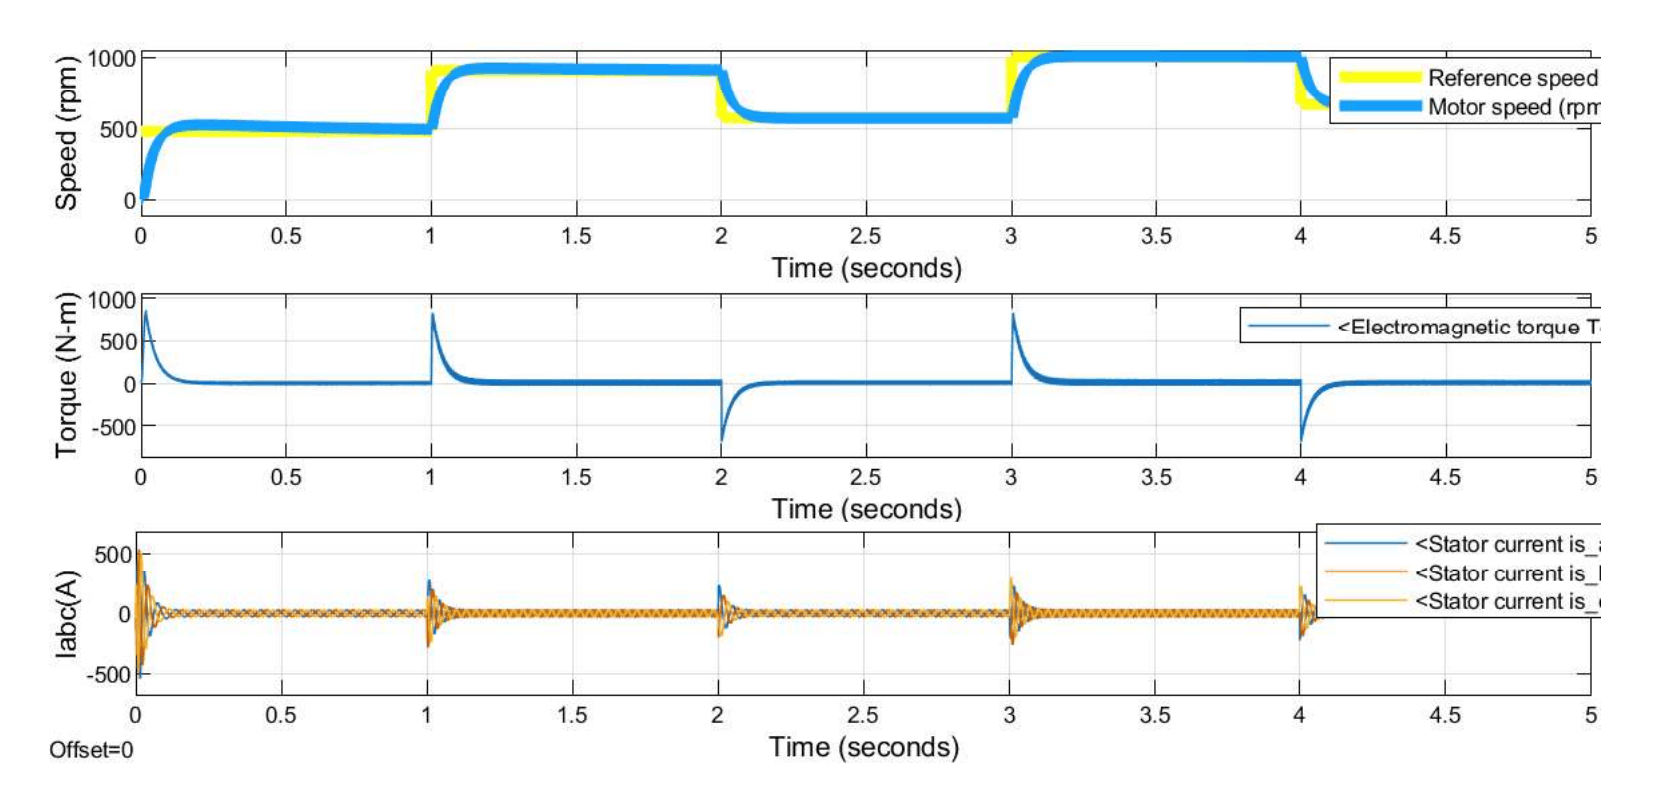
\includegraphics[width=0.8\textwidth]{7.png}
\caption{Dynamic Response of Motor Speed, Torque, and Phase Currents}
\end{figure}

\begin{figure}[H]
\centering
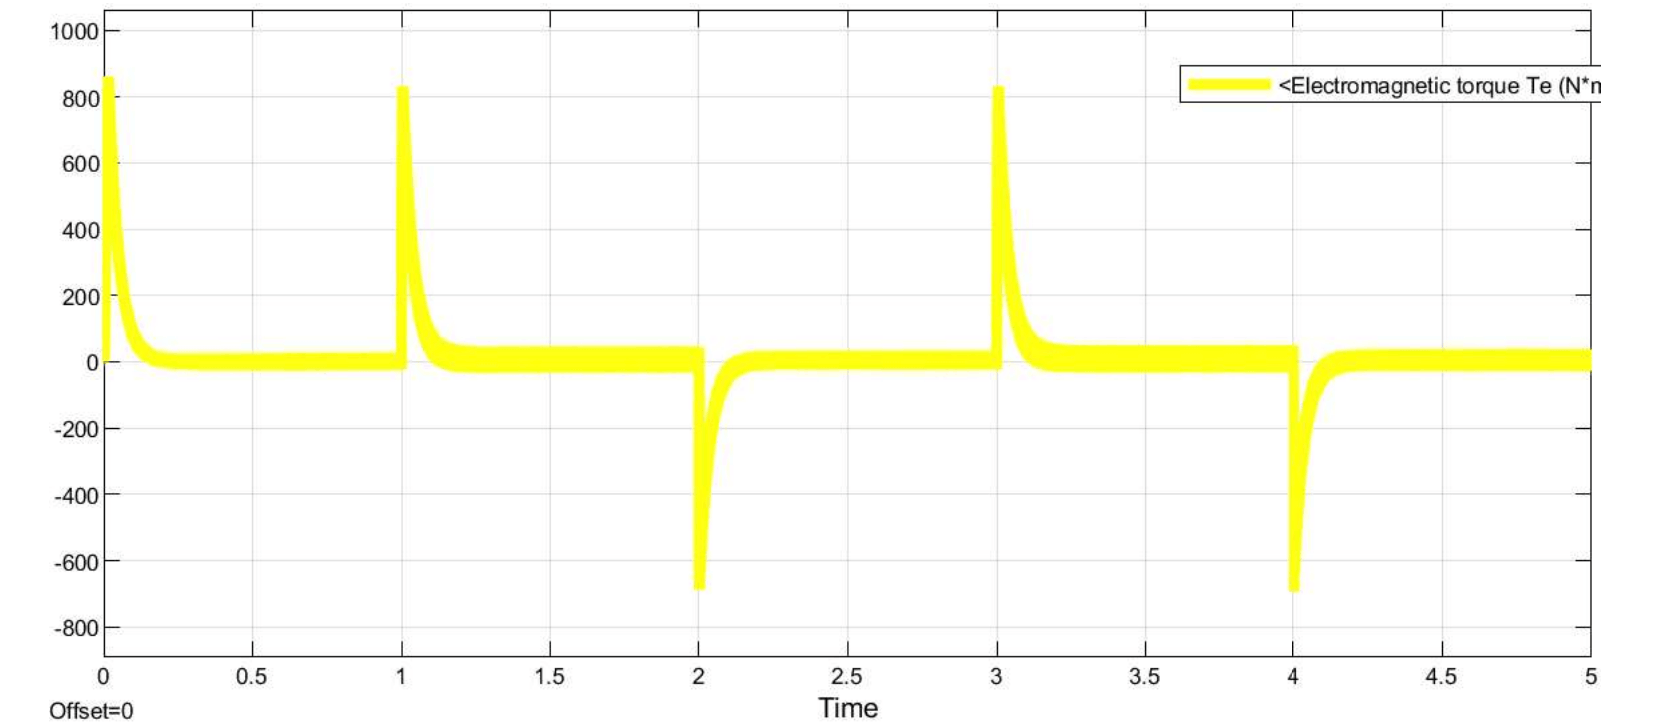
\includegraphics[width=0.8\textwidth]{1.png}
\caption{Electromagnetic Torque Transient Spikes during Acceleration/Deceleration}
\end{figure}

\begin{figure}[H]
\centering
\includegraphics[width=0.8\textwidth]{20.jpg}
\caption{Rotor Flux Estimation Reaching Steady State}
\end{figure}

\begin{figure}[H]
\centering
\includegraphics[width=0.8\textwidth]{22.jpg}
\caption{Stator $d$-axis and $q$-axis Currents ($I_{ds}$ and $I_{qs}$)}
\end{figure}

\begin{figure}[H]
\centering
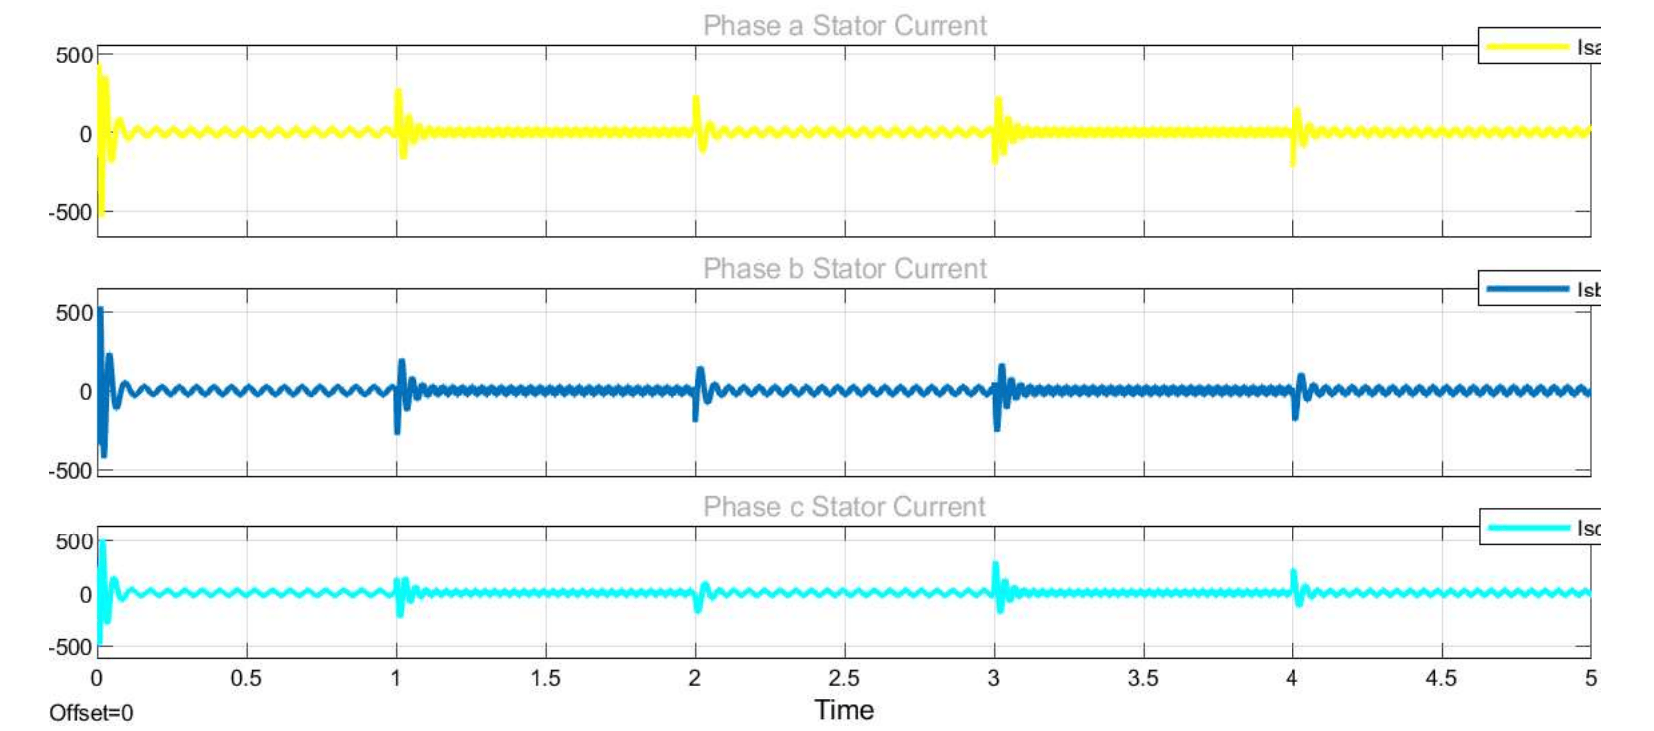
\includegraphics[width=0.8\textwidth]{23.png}
\caption{Three-Phase Stator Currents Under Dynamic Load Changes}
\end{figure}

\begin{figure}[H]
\centering
\includegraphics[width=0.8\textwidth]{24.jpg}
\caption{Induced Rotor Currents at Startup}
\end{figure}

\begin{figure}[H]
\centering
\includegraphics[width=0.8\textwidth]{15.jpg}
\caption{Steady-State Stator Voltages $V_d$ and $V_q$}
\end{figure}

\begin{figure}[H]
\centering
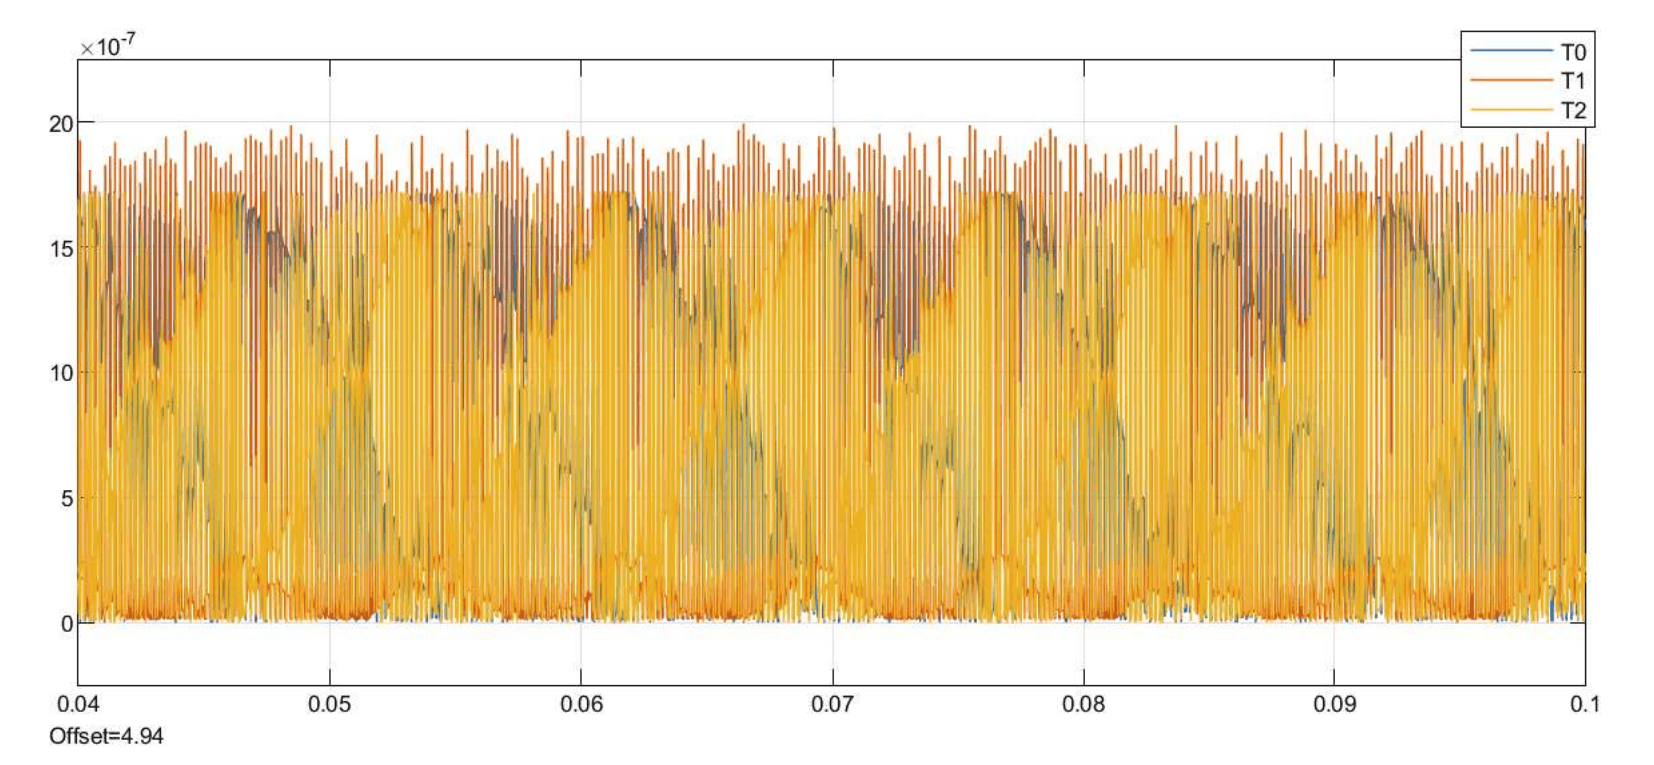
\includegraphics[width=0.8\textwidth]{31.png}
\caption{Calculated SVPWM Dwell Times ($T_0, T_1, T_2$)}
\end{figure}

\begin{figure}[H]
\centering
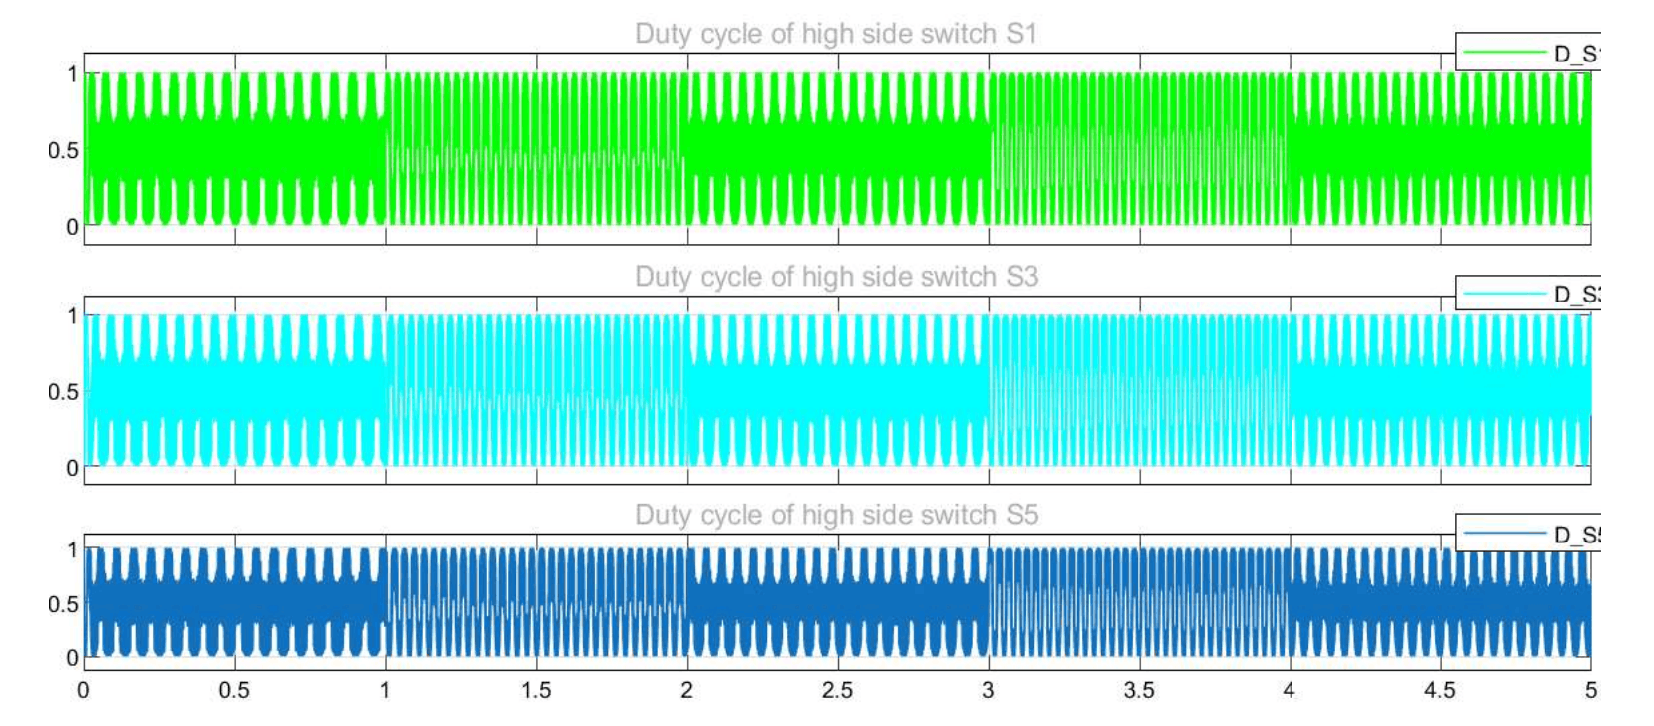
\includegraphics[width=0.8\textwidth]{32.png}
\caption{Duty Cycles for High-Side Inverter Switches ($S_1, S_3, S_5$)}
\end{figure}

\begin{figure}[H]
\centering
\includegraphics[width=0.8\textwidth]{34.jpg}
\caption{Final Discretized Gate Pulses for IGBTs}
\end{figure}

\begin{figure}[H]
\centering
\includegraphics[width=0.8\textwidth]{35.png}
\caption{Phase and Line Voltage Measurements on the Plant}
\end{figure}

Ultimately, this Simulink model serves as an instructional framework, unifying electromagnetic machine theory, advanced discrete-time control systems, and power electronic actuation.

\section{Future Scope}
The simulation foundation established in this report supports several future implementations. Work will focus on transitioning this model to physical hardware via Hardware-in-the-Loop (HIL) testing and deployment using a microcontroller such as the STM32 framework. Furthermore, integrating sensorless control estimators to replace the physical encoder would support system reliability, while the application of Model Predictive Control (MPC) could be investigated to address the limitations of traditional PI regulators.

% ---------------- BIBLIOGRAPHY ----------------
\chapter*{Bibliography}
\addcontentsline{toc}{chapter}{Bibliography}
\begin{enumerate}
    \item Texas Instruments, \textit{Sensorless Field Oriented Control of 3-Phase Induction Motors}, Application Report SPRABP9, 2013.
    \item Bose, B. K. \textit{Modern Power Electronics and AC Drives}. Prentice Hall PTR, 2001.
\end{enumerate}

\end{document}